%-*- program: xelatex -*-        
%-*- program: biber -*-`        
%-*- program: xelatex -*-
\documentclass[11pt]{article}
\usepackage[margin=0.75in]{geometry}            % See geometry.pdf to learn the layout options. There are lots.
\geometry{letterpaper}  
\usepackage{amsmath,textcomp,amssymb,geometry,graphicx,enumerate,upquote,color}
\usepackage{hyperref}
\usepackage{breqn}
\usepackage{float}
\usepackage{tikz}
\usepackage{array}
\usepackage{float}
\usepackage{amsfonts}
\def\Session{Fall 2015}
\usepackage[english]{babel}
\title{Drawdown Project - Simulation}
\author{Boying Gong, Xinyue Zhou}
\newenvironment{qparts}{\begin{enumerate}[{(}a{)}]}{\end{enumerate}}
\def\endproofmark{$\Box$}
\newenvironment{proof}{\par{\bf Proof}:}{\endproofmark\smallskip}
\begin{document}
\maketitle

\tableofcontents

\clearpage

\section{Noice term with normal distribution}

To better understand the behaviour of conditional expected drawdown (CED) and the maximum drawdown distribution, we use some simple assumptions and paramters in this section as follows:

\begin{enumerate}
\item Noice term in the time series model follows Normal distribution with standard deviation of 0.01: $\epsilon \sim N(0, 0.0001)$.
\item Risk measures including volatility, VaR, ES and maximum drawdown are calculated based on simulated time series with path length 1000. The calculation of maximum drawdown is replicated 1000 times in order to obtain the maximum drawdown distribution and its tail mean (CED).
\item All time series parameters in this section range from -0.9 to 0.9. For time series with multiple parameters such as AR(2), ARMA(1, 1), the parameters are cartesian product of arithmetic progressions range from -0.9 to 0.9. Note that to take the stationary of AR and ARMA models into consideration (all moving averages are stationary, but the AR and ARMA model have to meet certain criteria to be stationary), not all parameters in the cartesian product are used in the simulation.
\end{enumerate}

%%%%%%%%%%%%
\subsection{AR(1)} %%%%
%%%%%%%%%%%%

We started from the simplest model AR(1):

\begin{equation}
X_t = \kappa_1X_{t-1} + \epsilon_t
\end{equation}

We simulate AR(1) for various values of the autoregressive parameter for $\kappa_1 \in (-1, 1)$ . Figure \ref{fig:AR1_risk_measures} shows the relationship between AR(1) coefficient and risk measures of interest including ES, VaR, volatility and CED. Note that for AR(1) model, the order one serial correlation is the the value of autoregressive parameter.

CED shows a decreasing trend when $\kappa_1\in(-1, -0.75)$ and an increasing trend when $\kappa_1 \in(-0.75, 1)$. As shown in Figure \ref{fig:AR1_risk_measures}, it becomes feasible for us to distinguish negative and positive serial correlation using the CED values. However, the other 3 risk measures are all symmetric about $\kappa_1 = 0$, and they increase as the absolute values of $\kappa_1$ increases.

For VaR, ES and CED, the derivative of risk measure values to $\kappa_1$ approaches to zero as  $\kappa_1$ goes to 0 and increase as $\kappa_1$ increase. This suggests that the value of this three risk measures can hardly reflect the change of serial correlation when the serial correlation is small. And they perform better when the serial correlation increases. The trend of derivatives reverse for CED. While the change of $\kappa_1$ has a comparatively larger influence around 0, the influence becomes weaker as we move to larger  $\kappa_1$ values.

Figure \ref{fig:AR1_maxDrawdown_dist} shows the maximum drawdown distribution for various $\kappa_1$. Same as revealed in Figure \ref{fig:AR1_risk_measures}, the mean and tail mean of maximum drawdown distribution increases as we increase $\kappa_1$ from negative values to positive values.

Table \ref{table: AR1_return} shows the basic summary statistics of the simulated return sequences. The standard deviation increases as we increase the absolute values of the coefficient. The sknewness and kurtosis are close to zeros. Kolmogorov-Smirnov Tests indicate that they all follow normal distribution. 

\begin{figure}[H]
\centering
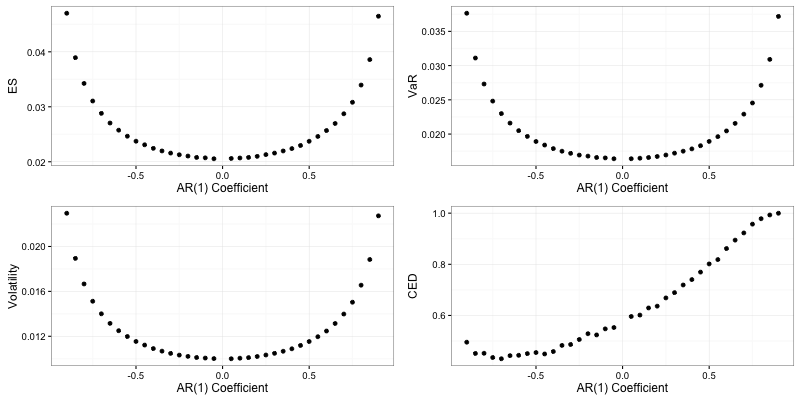
\includegraphics[width = 0.8\textwidth]{../figures/simulation/AR1_risk_measures}
\caption{AR(1): Relationship between auto-correlation coefficients and risk measures}
(Simulation path length: 1000, $\epsilon_t \sim N(0, 0.0001)$)
\label{fig:AR1_risk_measures}
\end{figure}

\begin{figure}[H]
\centering
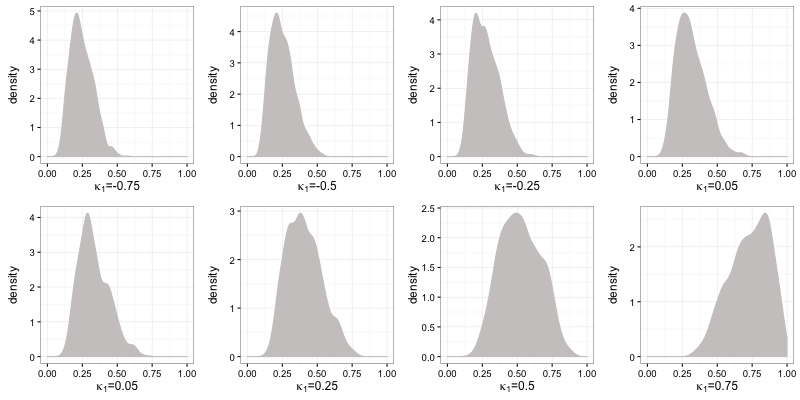
\includegraphics[width = 0.8\textwidth]{../figures/simulation/AR1_maxDrawdown_dist}
\caption{AR(1): Maximum drawdown distribution for various $\kappa_1$ values }
(Empirical distribution, path length = 1000, sample size = 1000, $\epsilon_t \sim N(0, 0.0001)$ )
\label{fig:AR1_maxDrawdown_dist}
\end{figure}

\begin{table}[H]
\centering
\begin{tabular}{|r |r r r r|}
\hline
& Mean & Sd & Sknewness & Kurtosis \\
\hline
$\kappa_1 = -0.75$ & 0.0 & 0.015 & 0.009 & 0.032\\
$\kappa_1 = -0.5$ & 0.0 & 0.012 & 0.006 & 0.021\\
$\kappa_1 = -0.25$ & 0.0 & 0.010 & 0.001 & 0.010\\
$\kappa_1 = 0.25$ & 0.0 & 0.010 & -0.009 & 0.004\\
$\kappa_1 = 0.5$ & 0.0 & 0.012 & -0.012 & -0.008\\
$\kappa_1 = 0.75$ & 0.0 & 0.015 & 0.013 & 0.016\\
\hline
\end{tabular}
\caption{Statistics of simulated distribution of AR(1)}
\label{table: AR1_return}
\end{table}

%%%%%%%%%%%%
\subsection{AR(2)} %%%%
%%%%%%%%%%%%

We then move to model AR(2):

\begin{equation}
X_t = \kappa_1X_{t-1} + \kappa_2X_{t-2}  + \epsilon_t
\end{equation}

Figure \ref{fig:AR2_risk_measures_pos} and \ref{fig:AR2_risk_measures_neg} shows the relationship between order one serial correlation $\rho_1$ and various risk measures. With fixed $\kappa_2$, the relationship between serial correlation and various risk measures are close to AR(1) model. The curve shows some discontinuity mainly because the stationary condition for which we have to drop some possible combination of coefficients. Nevertheless, Figure \ref{fig:AR2_risk_measures_pos} and \ref{fig:AR2_risk_measures_neg} shows more complexity in that as we increase the $\kappa_2$ value, the values of all four risk measures increases.

Figure \ref{fig:AR2_maxDrawdown_dist_kappa2_02} and \ref{fig:AR2_maxDrawdown_dist_kappa2_-02} shows the maximum drawdown distribution as we fix $\kappa_2$ to 0.2 and -0.2 respectively and change $\kappa_1$. Again the maximum drawdown distribution shows monotonicity as we increase $\kappa_1$ from negative to positive for both $\kappa_2 = 0.2 $ and $\kappa_2 = -0.2$. It would be the similar if we fix $\kappa_1$ and examine the maximum drawdown distribution for different $\kappa_2$ values.  

Table \ref{table: AR2_return} shows the summary statistics for the simulated return sequences. As indicated above, the standard deviation value increases as we increase the absolute values of the coefficient. The sknewness and kurtosis are close to zeros.

\begin{figure}[H]
\centering
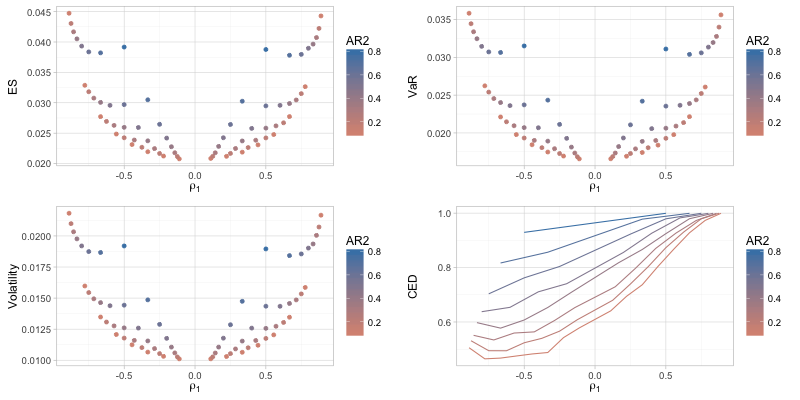
\includegraphics[width = 0.8\textwidth]{../figures/simulation/AR2_risk_measures_pos}
\caption{AR(2): Relationship between serial correlation $\rho_1$ and risk measures ($\kappa_2 > 0$)}
(Simulation path length: 1000, $\epsilon_t \sim N(0, 0.0001)$)
\label{fig:AR2_risk_measures_pos}
\end{figure}

\begin{figure}[H]
\centering
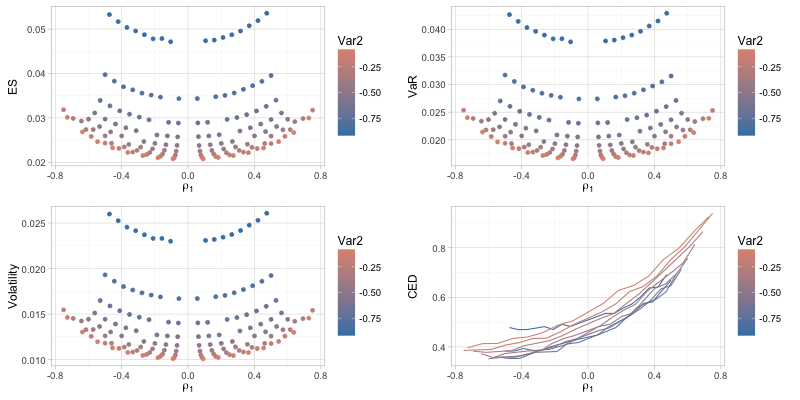
\includegraphics[width = 0.8\textwidth]{../figures/simulation/AR2_risk_measures_neg}
\caption{AR(2): Relationship between serial correlation $\rho_1$ and risk measures ($\kappa_2 < 0$)}
(Simulation path length: 1000, $\epsilon_t \sim N(0, 0.0001)$)
\label{fig:AR2_risk_measures_neg}
\end{figure}

\begin{figure}[H]
\centering
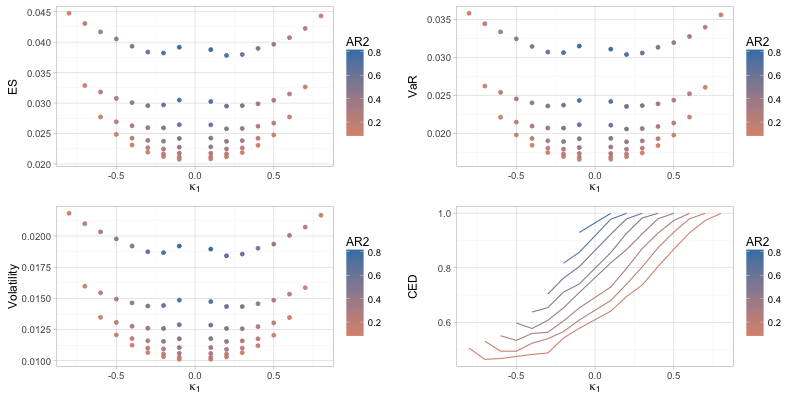
\includegraphics[width = 0.8\textwidth]{../figures/simulation/AR2_risk_measures_pos_coef}
\caption{AR(2): Relationship between model coefficients and risk measures ($\kappa_2 > 0$)}
(Simulation path length: 1000, $\epsilon_t \sim N(0, 0.0001)$)
\label{fig:AR2_risk_measures_pos_coef}
\end{figure}

\begin{figure}[H]
\centering
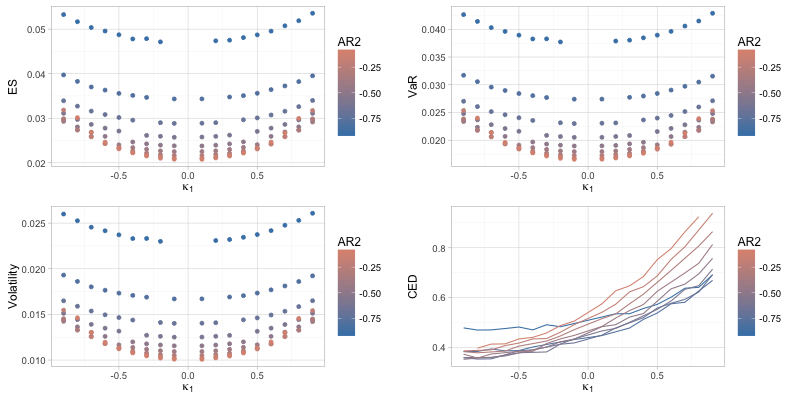
\includegraphics[width = 0.8\textwidth]{../figures/simulation/AR2_risk_measures_neg_coef}
\caption{AR(2): Relationship between model coefficientss and risk measures ($\kappa_2 < 0$)}
(Simulation path length: 1000, $\epsilon_t \sim N(0, 0.0001)$)
\label{fig:AR2_risk_measures_neg_coef}
\end{figure}

\begin{figure}[H]
\centering
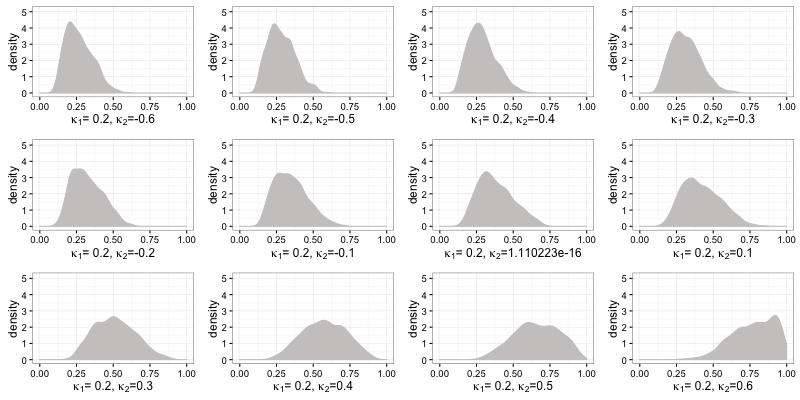
\includegraphics[width = 0.8\textwidth]{../figures/simulation/AR2_maxDrawdown_dist_kappa1_02}
\caption{AR(2): Maximum drawdown distribution for $\kappa_2 = 0.2$}
(Empirical distribution, path length = 1000, sample size = 1000, $\epsilon_t \sim N(0, 0.0001)$ )
\label{fig:AR2_maxDrawdown_dist_kappa2_02}
\end{figure}

\begin{figure}[H]
\centering
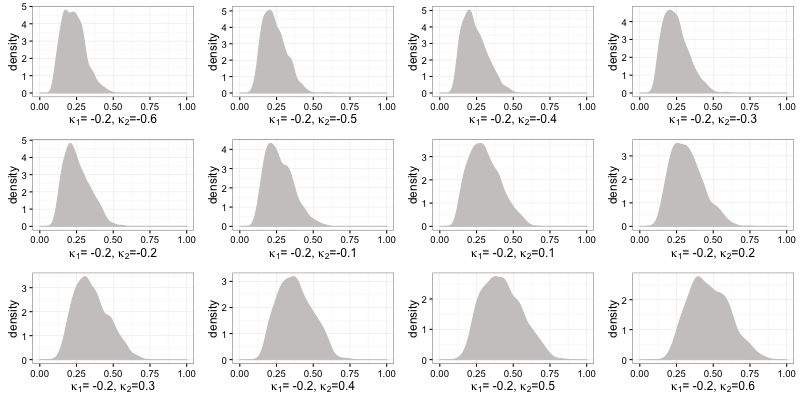
\includegraphics[width = 0.8\textwidth]{../figures/simulation/AR2_maxDrawdown_dist_kappa1_-02}
\caption{AR(2): Maximum drawdown distribution for $\kappa_ = -0.2$}
(Empirical distribution, path length = 1000, sample size = 1000, $\epsilon_t \sim N(0, 0.0001)$ )
\label{fig:AR2_maxDrawdown_dist_kappa2_-02}
\end{figure}

\begin{table}[H]
\centering
\begin{tabular}{|r |r r r r|}
\hline
& Mean & Sd & Sknewness & Kurtosis \\
\hline
$\kappa_1 = -0.75, \kappa_2 = 0.2$ & 0.0 & 0.029 & -0.005 & 0.039\\
$\kappa_1 = -0.5, \kappa_2 = 0.2$ & 0.0 & 0.013 & 0.000 & 0.004\\
$\kappa_1 = -0.25, \kappa_2 = 0.2$ & 0.0 & 0.011 & 0.003 & -0.021\\
$\kappa_1 = 0.25, \kappa_2 = 0.2$ & 0.0 &  0.011 & 0.003 & -0.008\\
$\kappa_1 = 0.5, \kappa_2 = 0.2$ & 0.0 & 0.013 & 0.012 & -0.010\\
$\kappa_1 = 0.75, \kappa_2 = 0.2$ & 0.0 &  0.029 & -0.001 & -0.021\\
\hline
\end{tabular}
\caption{Statistics of simulated distribution of AR(2)}
\label{table: AR2_return}
\end{table}

%%%%%%%%%%%%
\subsection{MA(1)} %%%%
%%%%%%%%%%%%

For simplest moving average model MA(1):

\begin{equation}
X_t = \epsilon_t + \theta_1\epsilon_{t-1}
\end{equation}

Figure \ref{fig:MA1_risk_measures_acf1} presents the relationship between four risk measures and serial correlation $\rho_1$. Similar with autoregressive models, CED is a informative risk measures for distinguish positive and negative serial correlations. The curve of $\rho_1$ versus CED is convex for positive serial correlation and concave for negative serial correlation. With means the rate of change of CED to $\rho_1$ is smaller for small serial correlation values and increases for larger serial correlation values. Figure \ref{fig:MA1_risk_measures_coefficient} shows the relationship between risk measures and the moving average coefficient $\theta_1$. Unlike Figure \ref{fig:MA1_risk_measures_acf1}, the MA(1) coefficient shows a relationship close to linear with the change of CED.

Figure \ref{fig:MA1_maxDrawdown_dist} shows the maximum drawdown distribution as we increase $\theta_1$. Same as revealed in the tail mean (CED) of the distribution. The maximum drawdown distribution monotonic increase as $\theta_1$ increases.

\begin{figure}[H]
\centering
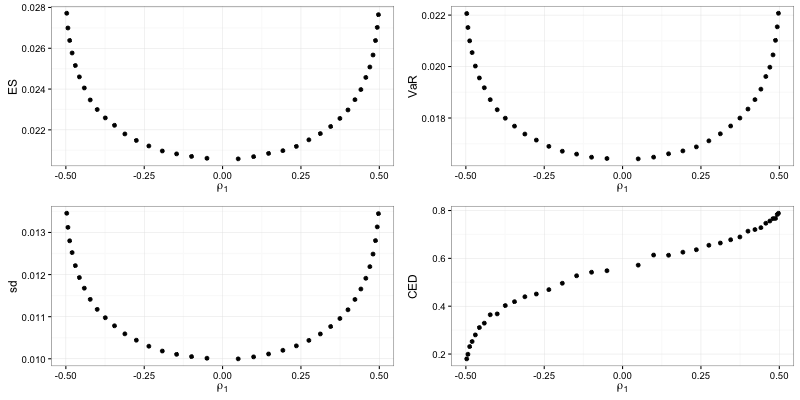
\includegraphics[width = 0.8\textwidth]{../figures/simulation/MA1_risk_measures_acf1}
\caption{MA(1): Relationship between serial correlation $\rho_1$ and risk measures}
(Simulation path length: 1000, $\epsilon_t \sim N(0, 0.0001)$)
\label{fig:MA1_risk_measures_acf1}
\end{figure}

\begin{figure}[H]
\centering
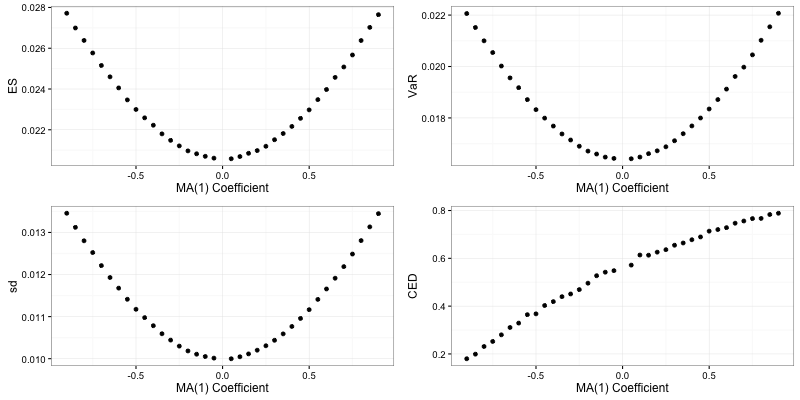
\includegraphics[width = 0.8\textwidth]{../figures/simulation/MA1_risk_measures_coefficient}
\caption{MA(1): Relationship between model coefficient and risk measures}
(Simulation path length: 1000, $\epsilon_t \sim N(0, 0.0001)$)
\label{fig:MA1_risk_measures_coefficient}
\end{figure} 

\begin{figure}[H]
\centering
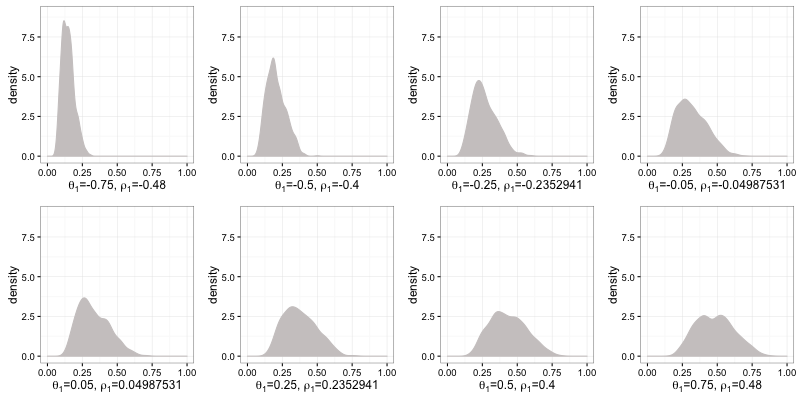
\includegraphics[width = 0.8\textwidth]{../figures/simulation/MA1_maxDrawdown_dist}
\caption{MA(1): Maximum drawdown distribution for various $\theta_1$ values}
(Empirical distribution, path length = 1000, sample size = 1000, $\epsilon_t \sim N(0, 0.0001)$ )
\label{fig:MA1_maxDrawdown_dist}
\end{figure}

\begin{table}[H]
\centering
\begin{tabular}{|r |r r r r|}
\hline
& Mean & Sd & Sknewness & Kurtosis \\
\hline
$\theta_1 = -0.75$ & 0.0 & 0.012 & -0.002 & -0.008\\
$\theta_1 = -0.5$ & 0.0 & 0.011 & -0.004 & -0.009\\
$\theta_1 = -0.25$ & 0.0 &  0.010 &  0.001 & -0.020\\
$\theta_1 = 0.25$ & 0.0 &  0.010 & 0.011 & 0.023\\
$\theta_1 = 0.5$ & 0.0 & 0.011 & 0.000 & 0.006\\
$\theta_1 = 0.75$ & 0.0 & 0.013 & -0.003 & 0.012\\
\hline
\end{tabular}
\caption{Statistics of simulated distribution of MA(1)}
\label{table: MA1_return}
\end{table}

%%%%%%%%%%%%%%%%%%%%%%%%
\subsection{MA(2)} %%%%
%%%%%%%%%%%%%%%%%%%%%%%%

The expression of MA(2) model is:

\begin{equation}
X_t = \epsilon_t + \theta_1\epsilon_{t-1} + \theta_2\epsilon_{t-2}
\end{equation}

As shown in Figure \ref{fig:MA2_risk_measures_pos} and Figure \ref{fig:AR2_risk_measures_neg}, when fix $\theta_2$, the relationship between serial correlation $\rho_1$ and risk measures resembles that of the MA(1) model. When we increase the absolute values of $\rho_2$, the value of ES, VaR and volatility increases. However, there are more complicated relationship between serial correlation and CED. For positive $\theta_2$, CED increase as $\theta_2$ increases. The pattern seems less interpretable for negative $\theta_2$ values. 

Figure \ref{fig:MA2_maxDrawdown_dist_theta1_02} shows the change of maximum drawdown distribution when we fix $\theta_1=0.2$, and Figure \ref{fig:MA2_maxDrawdown_dist_theta2_02} shows the maximum drawdown distribution when we fix $\theta_2=0.2$. When fixing one parameter and change the other parameter value from negative to positive, the maximum drawdown distributions are monotonic increasing, which indicates that the tail mean of the distribution (CED) increases.

Same as the AR(1), AR(2), and MA(1) model above, the mean, sknewness and kurtosis is small for our simulated return sequences. The standard deviation increase as we increase the absolute value of the coefficient, which can be explained by the theoretical calculation.

\begin{figure}[H]
\centering
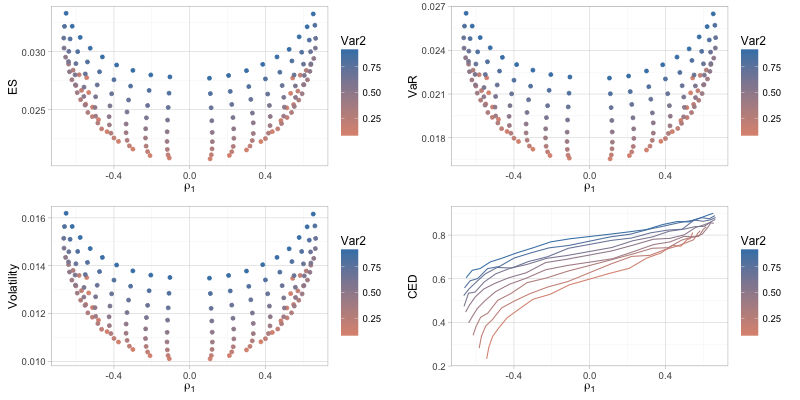
\includegraphics[width = 0.8\textwidth]{../figures/simulation/MA2_risk_measures_pos}
\caption{MA(2): Relationship between serial correlation $\rho_1$ and risk measures ($\theta_2>0$)}
(Simulation path length: 1000, $\epsilon_t \sim N(0, 0.0001)$)
\label{fig:MA2_risk_measures_pos}
\end{figure}

\begin{figure}[H]
\centering
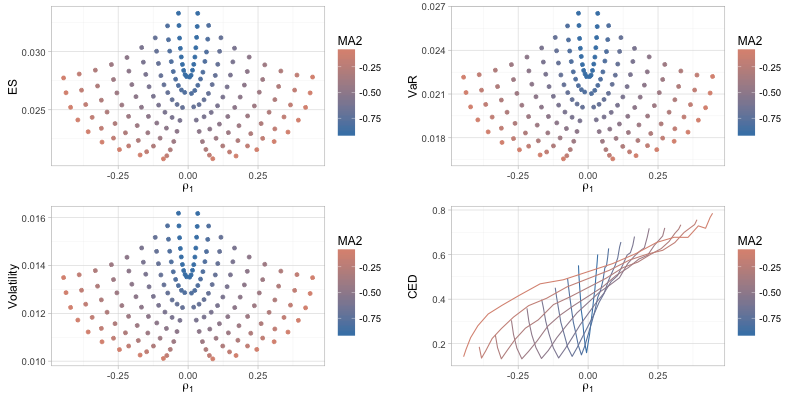
\includegraphics[width = 0.8\textwidth]{../figures/simulation/MA2_risk_measures_neg}
\caption{MA(2): Relationship between serial correlation $\rho_1$ and risk measures ($\theta_2<0$)}
(Simulation path length: 1000, $\epsilon_t \sim N(0, 0.0001)$)
\label{fig:MA2_risk_measures_neg}
\end{figure}

\begin{figure}[H]
\centering
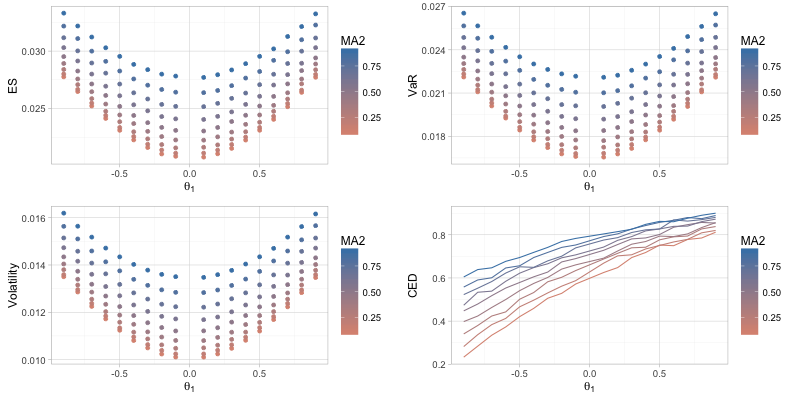
\includegraphics[width = 0.8\textwidth]{../figures/simulation/MA2_risk_measures_pos_coef}
\caption{MA(2): Relationship between model coefficients and risk measures ($\theta_2>0$)}
(Simulation path length: 1000, $\epsilon_t \sim N(0, 0.0001)$)
\label{fig:MA2_risk_measures_pos_coef}
\end{figure}

\begin{figure}[H]
\centering
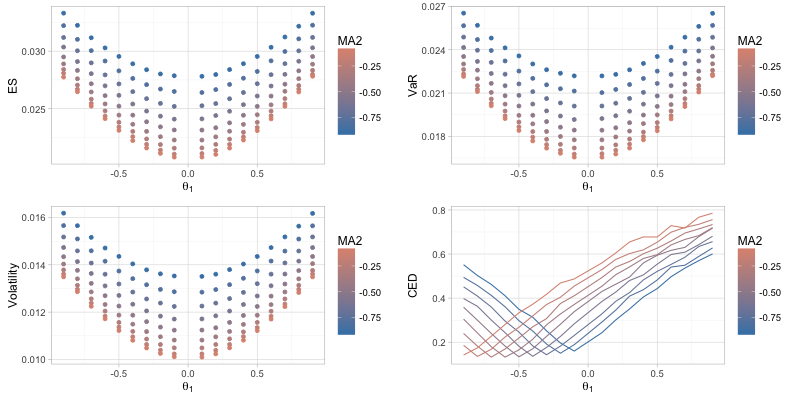
\includegraphics[width = 0.8\textwidth]{../figures/simulation/MA2_risk_measures_neg_coef}
\caption{MA(2): Relationship between model coefficients and risk measures ($\theta_2<0$)}
(Simulation path length: 1000, $\epsilon_t \sim N(0, 0.0001)$)
\label{fig:MA2_risk_measures_neg_coef}
\end{figure}

\begin{figure}[H]
\centering
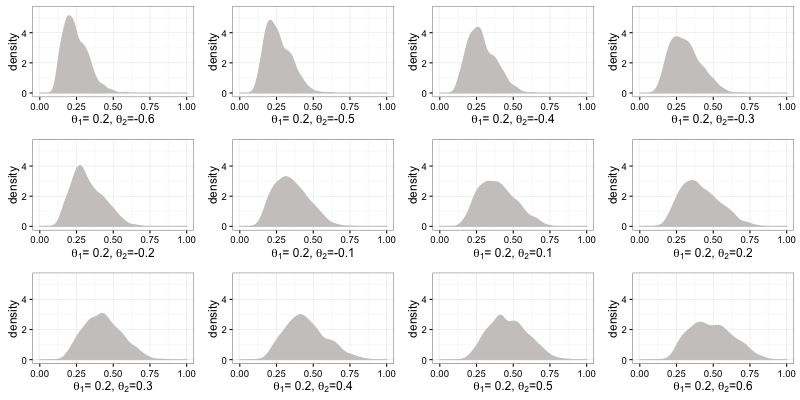
\includegraphics[width = 0.8\textwidth]{../figures/simulation/MA2_maxDrawdown_dist_theta1_02}
\caption{MA(2): Maximum drawdown distribution for $\theta_1 = 0.2$}
(Empirical distribution, path length = 1000, sample size = 1000, $\epsilon_t \sim N(0, 0.0001)$ )
\label{fig:MA2_maxDrawdown_dist_theta1_02}
\end{figure}

\begin{figure}[H]
\centering
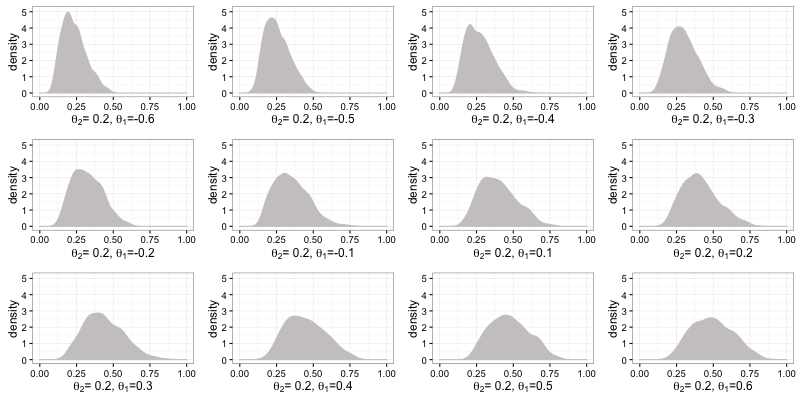
\includegraphics[width = 0.8\textwidth]{../figures/simulation/MA2_maxDrawdown_dist_theta2_02}
\caption{MA(2): Maximum drawdown distribution for $\theta_2 = 0.2$}
(Empirical distribution, path length = 1000, sample size = 1000, $\epsilon_t \sim N(0, 0.0001)$ )
\label{fig:MA2_maxDrawdown_dist_theta2_02}
\end{figure}

\begin{table}[H]
\centering
\begin{tabular}{|r |r r r r|}
\hline
& Mean & Sd & Sknewness & Kurtosis \\
\hline
$\theta_1 = -0.75, \theta_2 = 0.2$ & 0.0 & 0.013 & 0.004 & -0.015\\
$\theta_1 = -0.5, \theta_2 = 0.2$ & 0.0 & 0.011 & -0.006 & -0.002\\
$\theta_1 = -0.25, \theta_2 = 0.2$ & 0.0 &  0.011 & -0.004 & -0.012\\
$\theta_1 = 0.25, \theta_2 = 0.2$ & 0.0 &  0.010 & -0.020 & -0.007\\
$\theta_1 = 0.5, \theta_2 = 0.2$ & 0.0 & 0.011 & 0.009 & 0.012\\
$\theta_1 = 0.75, \theta_2 = 0.2$ & 0.0 & 0.013 & -0.015 & 0.025\\
\hline
\end{tabular}
\caption{Statistics of simulated distribution of MA(2)}
\label{table: MA2_return}
\end{table}

%%%%%%%%%%%%%%%%%%%%%%%%%
\subsection{ARMA(1, 1)} %%%%
%%%%%%%%%%%%%%%%%%%%%%%%%

For the most simple ARMA model:

\begin{equation}
X_t = \kappa_1X_{t-1} + \epsilon_t + \theta_1\epsilon_{t-1}
\end{equation}

Figure \ref{fig:AR1MA1_risk_measures_pos} and Figure Figure \ref{fig:AR1MA1_risk_measures_neg} shows the relationship between serial correlation $\rho_1$ and risk measures for positive and negative $\theta_1$ respectively. For positive $\theta_1$, the time series is more likely to be positively correlated while for negative $\theta_1$ it is mode likely to be negative correlated. Interestingly, for positive $\theta_1$ values, the relationship between CED and serial correlation $\rho_1$ is not influenced by the value of $\rho_1$. CED shows an increasing trend as we increase the value of serial correlation. Similar as the above subsections for other time series models, CED is a good tool to distinguish the postitive and negative seiral correlation.

\begin{figure}[H]
\centering
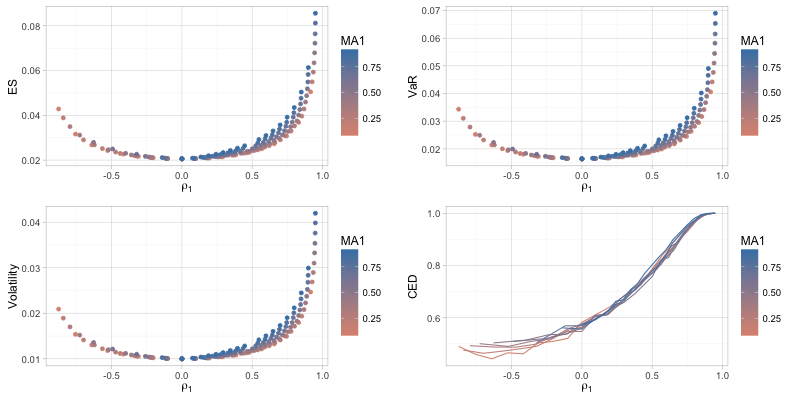
\includegraphics[width = 0.8\textwidth]{../figures/simulation/AR1MA1_risk_measures_pos}
\caption{ARMA(1, 1): Relationship between serial correlation $\rho_1$ and risk measures ($\theta_1>0$)}
(Simulation path length: 1000, $\epsilon_t \sim N(0, 0.0001)$)
\label{fig:AR1MA1_risk_measures_pos}
\end{figure}

\begin{figure}[H]
\centering
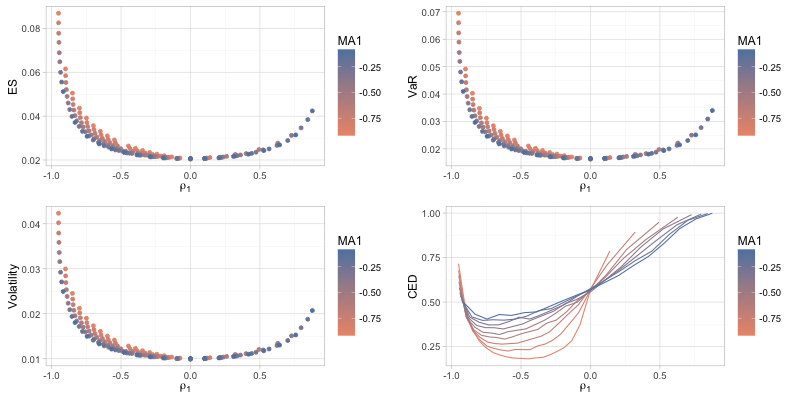
\includegraphics[width = 0.8\textwidth]{../figures/simulation/AR1MA1_risk_measures_neg}
\caption{ARMA(1, 1): Relationship between serial correlation $\rho_1$ and risk measures ($\theta_1>0$)}
(Simulation path length: 1000, $\epsilon_t \sim N(0, 0.0001)$)
\label{fig:AR1MA1_risk_measures_neg}
\end{figure}

\begin{figure}[H]
\centering
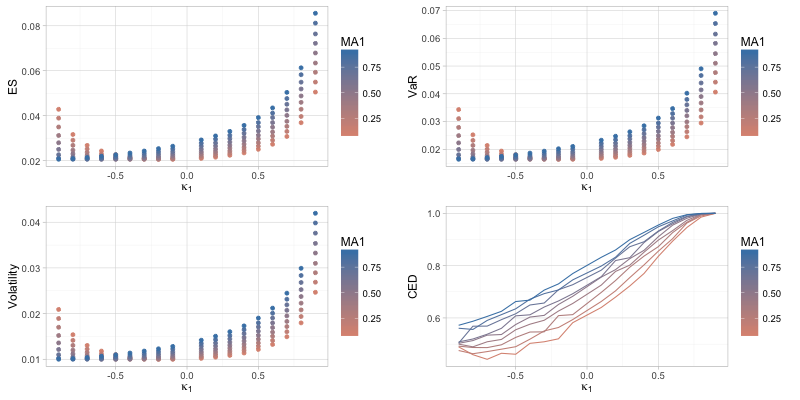
\includegraphics[width = 0.8\textwidth]{../figures/simulation/AR1MA1_risk_measures_pos_coef}
\caption{ARMA(1, 1): Relationship between model coefficient and risk measures ($\theta_1>0$)}
(Simulation path length: 1000, $\epsilon_t \sim N(0, 0.0001)$)
\label{fig:AR1MA1_risk_measures_pos_coef}
\end{figure}

\begin{figure}[H]
\centering
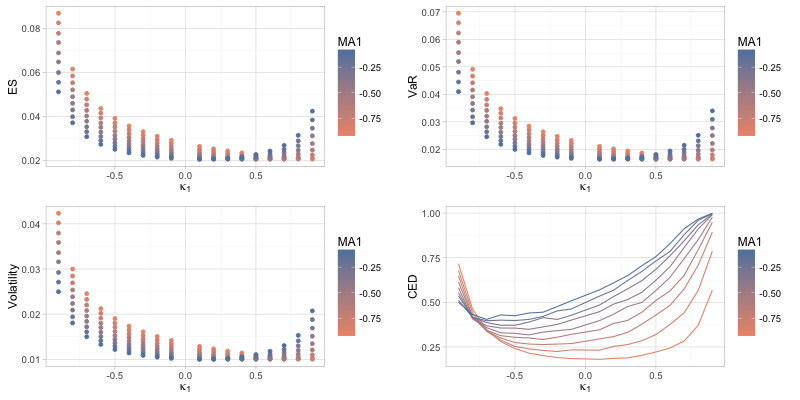
\includegraphics[width = 0.8\textwidth]{../figures/simulation/AR1MA1_risk_measures_neg_coef}
\caption{ARMA(1, 1): Relationship between model coefficient and risk measures ($\theta_1>0$)}
(Simulation path length: 1000, $\epsilon_t \sim N(0, 0.0001)$)
\label{fig:AR1MA1_risk_measures_neg_coef}
\end{figure}



%%%%%%%%%%%%%%%%%%%%%%%%%%%%%%%%%%%%%%%%%%%%%%%%%%
%%%%%%%%%%%%%%%%%%%%%%%%%%%%%%%%%%%%%%%%%%%%%%%%%%

\section{Noice term with student t distribution}

In this section, parameters used are close to what we've encountered in the empirical studies. 
\begin{enumerate}
\item White noice terms are simulated using t-distribution (degree of freedom = 4). Finanical return usually have fat-tail distributions.
\item Set path length to 63, which is the number of trading days in three month.
\item Time series parameters all range from -0.3 to 0.3, which is similar to the financial time series data in the real world. Usually financial data does not show strong serial correlation. If we could narrow down our scope to smaller serial correlations we may found that the serial correlation is more closely related with vaious risk measures.
\end{enumerate}

The relationship between serial correlation and risk measures revealed in this section resembles that of the last section where noice terms follow normal distribution. There are some differences due to the heavy-tail distribution. We illustrate more in the specific model part.

\subsection{AR(1)}

Models using time series with t-distribution white noice show more randomness as shown in Figure \ref{table: T_dist_AR1_return}. The relationship between AR(1) coefficients (which is the serial correlation $\rho_1$) and risk measures is similar to the model with normal distribution. However, the points are not lies prefectly in a curve probably bacause the heavy tail introduce more randomness of the quantile and tail mean values. 

Table \ref{table: T_dist_AR1_return} shows the summary statisitcs of the simulated return distribution. Their mean and skewness are close to zeor. And they have high kurtosis which implies the fat tail.

\begin{figure}[H]
\centering
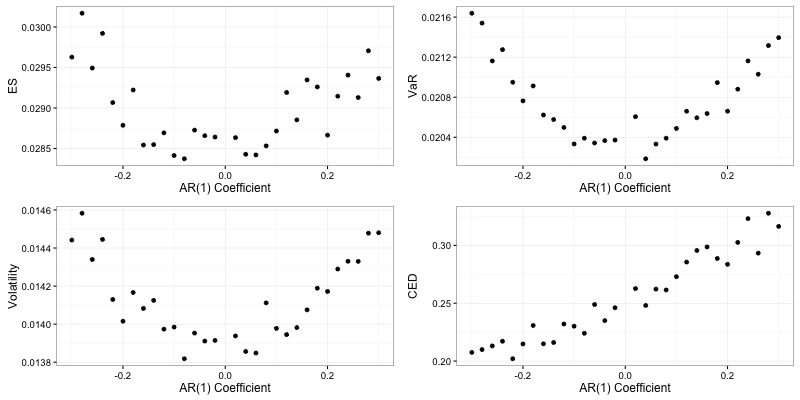
\includegraphics[width = 0.8\textwidth]{../figures/simulation/T_dist_AR1_risk_measures}
\caption{AR(1): Relationship between auto-correlation coefficients and risk measures}
(Simulation path length: 63, $\epsilon_t \sim 0.01T(df = 4)$)
\label{fig:T_dist_AR1_risk_measures}
\end{figure}



\begin{figure}[H]
\centering
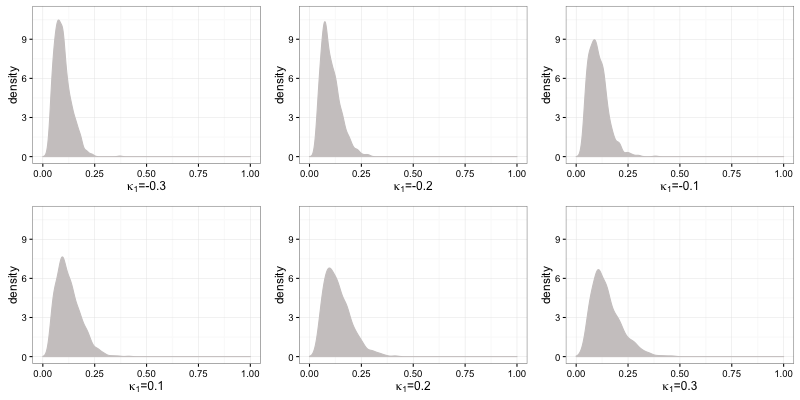
\includegraphics[width = 0.8\textwidth]{../figures/simulation/T_dist_AR1_maxDrawdown_dist}
\caption{AR(1): Maximum drawdown distribution for various $\kappa_1$ values }
(Empirical distribution, path length = 63, sample size = 1000, $\epsilon_t \sim 0.01T(df = 4)$)
\label{fig:T_dist_AR1_maxDrawdown_dist}
\end{figure}


\begin{table}[H]
\centering
\begin{tabular}{|r |r r r r|}
\hline
& Mean & Sd & Sknewness & Kurtosis \\
\hline
$\kappa_1 = -0.3$ & 0.0 & 0.015 & -0.53 & 18.8\\
$\kappa_1 = -0.2$ & 0.0 & 0.014 & -0.13 & 6.4\\
$\kappa_1 = -0.1$ & 0.0 & 0.014 & -0.05 & 6.3\\
$\kappa_1 = 0.1$ & 0.0 & 0.014 & -0.30 & 15.8\\
$\kappa_1 = 0.2$ & 0.0 & 0.014 & 0.13 & 7.0\\
$\kappa_1 = 0.3$ & 0.0 & 0.015 & -0.06 & 7.4\\
\hline
\end{tabular}
\caption{Statistics of simulated distribution of AR(1)}
\label{table: T_dist_AR1_return}
\end{table}

\subsection{AR(2)}

Same as presented in the last section, ES, VaR and volatility increases as we increase the absolute values of $\kappa_2$. And CED increases as we change $\kappa_2$ from negative to positive. This shows that CED values are inherently not symmetric not only for the serial correlation but for the coefficents. The summary statistics in Table \ref{table: T_dist_AR2_return} also indicate the fat tail distribution.

\begin{figure}[H]
\centering
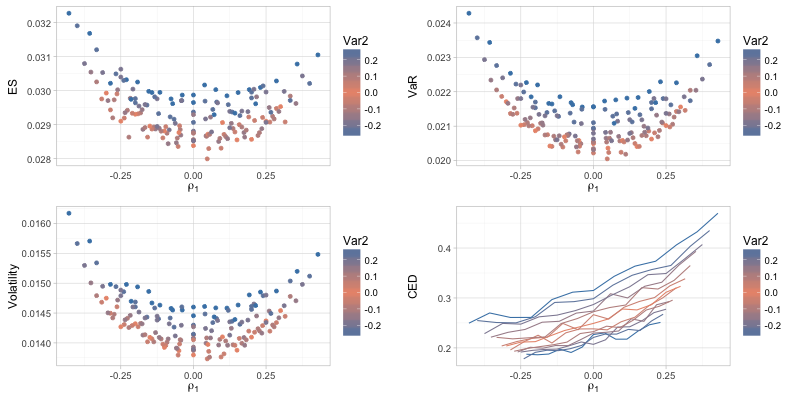
\includegraphics[width = 0.8\textwidth]{../figures/simulation/T_dist_AR2_risk_measures}
\caption{AR(2): Relationship between auto-correlation coefficients and risk measures}
(Simulation path length: 63, $\epsilon_t \sim 0.01T(df = 4)$)
\label{fig:T_dist_AR2_risk_measures}
\end{figure}

\begin{figure}[H]
\centering
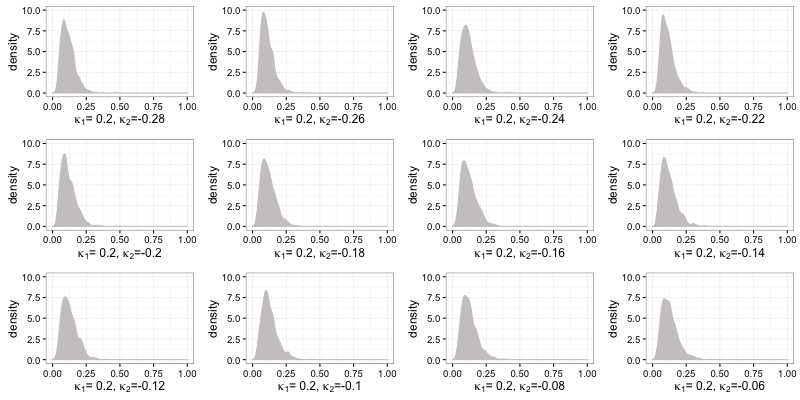
\includegraphics[width = 0.8\textwidth]{../figures/simulation/T_dist_AR2_maxDrawdown_dist_kappa1_02}
\caption{AR(2): Maximum drawdown distribution for various $\kappa_2$ values }
(Empirical distribution, path length = 63, sample size = 1000, $\epsilon_t \sim 0.01T(df = 4)$)
\label{fig:T_dist_AR2_maxDrawdown_dist_kappa1_02}
\end{figure}

\begin{table}[H]
\centering
\begin{tabular}{|r |r r r r|}
\hline
& Mean & Sd & Sknewness & Kurtosis \\
\hline
$\kappa_1 = 0.1, \kappa_2 = -0.3$ & 0.0 & 0.015 & -0.024 & 16.7\\
$\kappa_1 = 0.1, \kappa_2 = -0.2$ & 0.0 & 0.014 & -0.030 & 8.0\\
$\kappa_1 = 0.1, \kappa_2 = -0.1$ & 0.0 & 0.014 & -0.261 & 16.7\\
$\kappa_1 = 0.1, \kappa_2 = 0.1$ & 0.0 & 0.014 & -0.461 & 18.2\\
$\kappa_1 = 0.1, \kappa_2 = 0.2$ & 0.0 & 0.014 & 0.028 & 6.0\\
$\kappa_1 = 0.1, \kappa_2 = 0.3$ & 0.0 & 0.015 & -0.009 & 5.8\\
\hline
\end{tabular}
\caption{Statistics of simulated distribution of AR(2)}
\label{table: T_dist_AR2_return}
\end{table}

\subsection{MA(1)}

Again the relationship between serial correlation and risk measures for MA(1) model greatly resembles the relationship in last section for the normal distributed noice term. The difference lies in the large randomness caused by the fat tail. 

\begin{figure}[H]
\centering
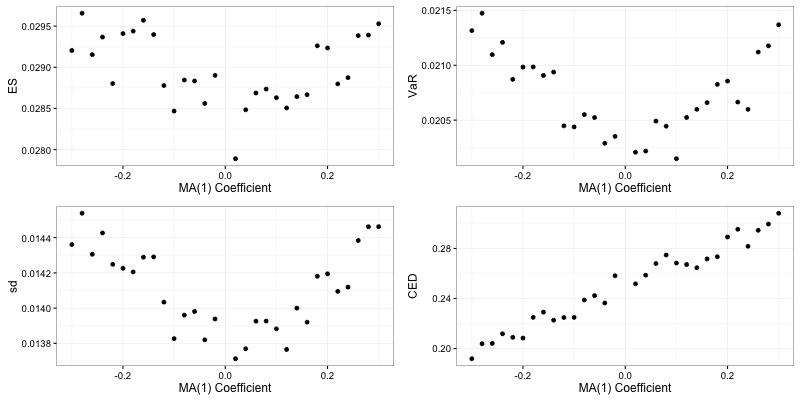
\includegraphics[width = 0.8\textwidth]{../figures/simulation/T_dist_MA1_risk_measures_coefficient.png}
\caption{MA(1): Relationship between serial correlation $\rho_1$ and risk measures}
(Simulation path length: 63, $\epsilon_t \sim 0.01T(df = 4)$)
\label{fig:T_dist_MA1_risk_measures_coefficient}
\end{figure}

\begin{figure}[H]
\centering
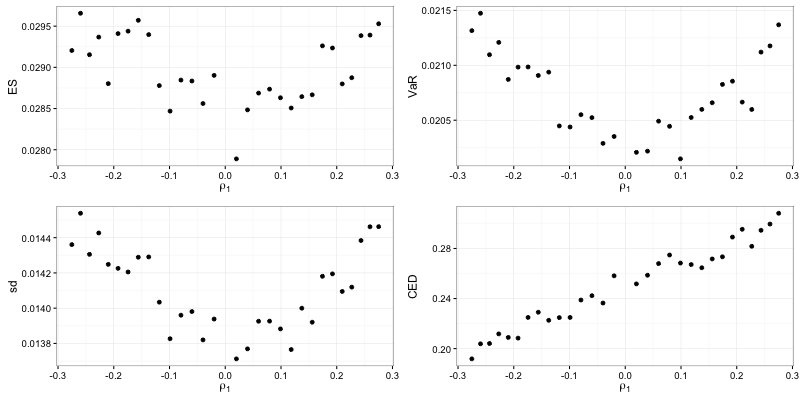
\includegraphics[width = 0.8\textwidth]{../figures/simulation/T_dist_MA1_risk_measures_acf1.png}
\caption{MA(1): Relationship between model coefficient and risk measures}
(Simulation path length: 63, $\epsilon_t \sim 0.01T(df = 4)$)
\label{fig:T_dist_MA1_risk_measures_acf1}
\end{figure} 

\begin{figure}[H]
\centering
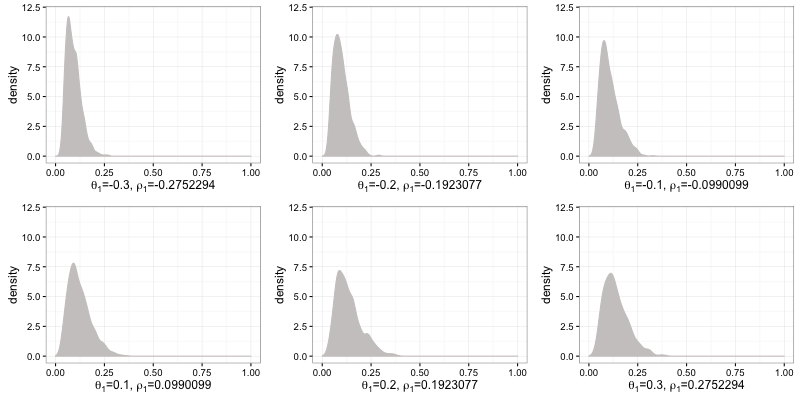
\includegraphics[width = 0.8\textwidth]{../figures/simulation/T_dist_MA1_maxDrawdown_dist}
\caption{MA(1): Maximum drawdown distribution for various $\kappa_1$ values }
(Empirical distribution, path length = 63, sample size = 1000, $\epsilon_t \sim 0.01T(df = 4)$)
\label{fig:T_dist_MA1_maxDrawdown_dist}
\end{figure}

\begin{table}[H]
\centering
\begin{tabular}{|r |r r r r|}
\hline
& Mean & Sd & Sknewness & Kurtosis \\
\hline
$\kappa_1 = 0.1, \kappa_2 = -0.3$ & 0.0 & 0.015 & -0.401 & 22.9\\
$\kappa_1 = 0.1, \kappa_2 = -0.2$ & 0.0 & 0.014 & -0.312 & 12.3\\
$\kappa_1 = 0.1, \kappa_2 = -0.1$ & 0.0 & 0.014 & -0.204 & 8.5\\
$\kappa_1 = 0.1, \kappa_2 = 0.1$ & 0.0 & 0.014 & -0.009 & 9.7\\
$\kappa_1 = 0.1, \kappa_2 = 0.2$ & 0.0 & 0.014 & -0.080 & 7.2\\
$\kappa_1 = 0.1, \kappa_2 = 0.3$ & 0.0 & 0.015 & -0.136 & 12.5\\
\hline
\end{tabular}
\caption{Statistics of simulated distribution of MA(1)}
\label{table: T_dist_MA1_return}
\end{table}

\subsection{MA(2)}

Since we have narrowed down our scope to time series coefficients which range between -0.3 and 0.3. Here we can see that for fixed value of $\theta_2$, the relationship between serial correlation and CED is approximately a line. And for the other three risk measures, the relationship seems to have more randomness than using normal distribution. 

\begin{figure}[H]
\centering
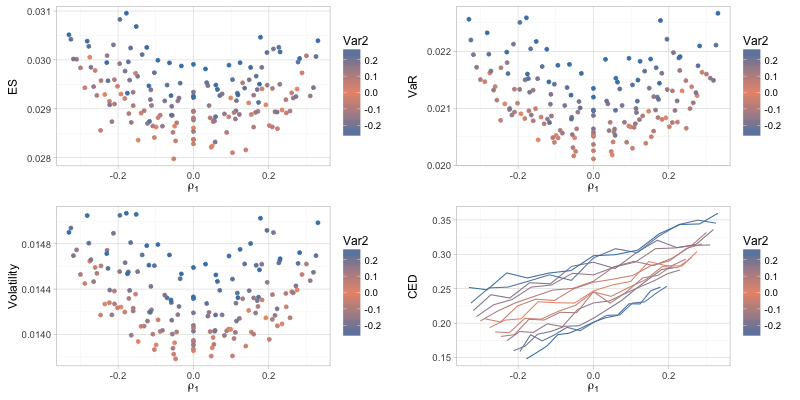
\includegraphics[width = 0.8\textwidth]{../figures/simulation/T_dist_MA2_risk_measures}
\caption{MA(1): Relationship between serial correlation $\rho_1$ and risk measures}
(Simulation path length: 63, $\epsilon_t \sim 0.01T(df = 4)$)
\label{fig:T_dist_MA2_risk_measures}
\end{figure}

\begin{figure}[H]
\centering
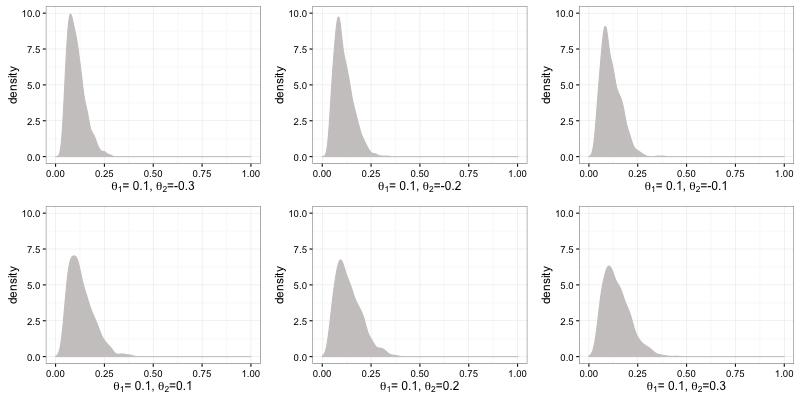
\includegraphics[width = 0.8\textwidth]{../figures/simulation/T_dist_MA2_maxDrawdown_dist_theta1_01}
\caption{MA(1): Maximum drawdown distribution for various $\kappa_1$ values }
(Empirical distribution, path length = 63, sample size = 1000, $\epsilon_t \sim 0.01T(df = 4)$)
\label{fig:T_dist_MA2_maxDrawdown_dist_theta1_01.png}
\end{figure}

\begin{table}[H]
\centering
\begin{tabular}{|r |r r r r|}
\hline
& Mean & Sd & Sknewness & Kurtosis \\
\hline
$\kappa_1 = 0.1, \kappa_2 = -0.3$ & 0.0 & 0.015 & -0.204 & 10.7\\
$\kappa_1 = 0.1, \kappa_2 = -0.2$ & 0.0 & 0.015 & 0.162 & 8.9\\
$\kappa_1 = 0.1, \kappa_2 = -0.1$ & 0.0 & 0.014 & -0.229 & 6.2\\
$\kappa_1 = 0.1, \kappa_2 = 0.1$ & 0.0 & 0.014 & -0.220 & 13.3\\
$\kappa_1 = 0.1, \kappa_2 = 0.2$ & 0.0 & 0.015 & 0.117 & 9.7\\
$\kappa_1 = 0.1, \kappa_2 = 0.3$ & 0.0 & 0.015 & -0.097 & 9.9\\
\hline
\end{tabular}
\caption{Statistics of simulated distribution of MA(2)}
\label{table: T_dist_MA2_return}
\end{table}

\subsection{ARMA(1, 1)}

\begin{figure}[H]
\centering
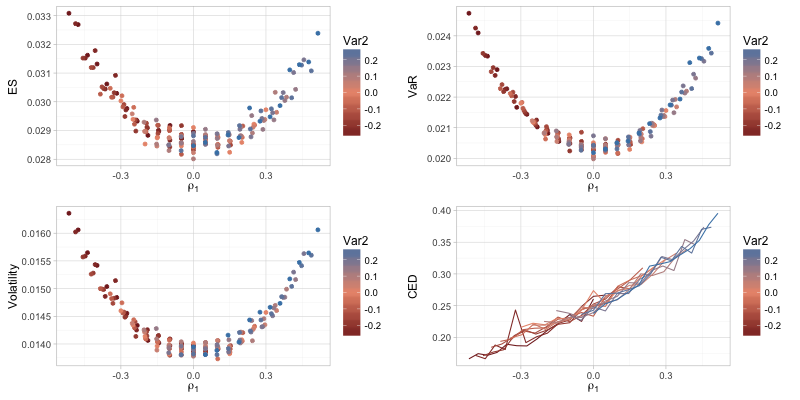
\includegraphics[width = 0.8\textwidth]{../figures/simulation/T_dist_AR1MA1_risk_measures}
\caption{ARMA(1, 1): Relationship between serial correlation $\rho_1$ and risk measures}
(Simulation path length: 63, $\epsilon_t \sim 0.01T(df = 4)$)
\label{fig:T_dist_AR1MA1_risk_measures}
\end{figure}

%%%%%%%%%%%%%%%%%%%%%%%%%
\section{Thoughts}  %%%%%
%%%%%%%%%%%%%%%%%%%%%%%%%

The relationship between serial correlation is complicated even for simple models such as AR(2), MA(2) and ARMA(1, 1). We tried several ways to present the relationship. Plots in this report are the best we came up with.

We did not move to more sophisticated time series models with higher orders. The patterns in some sense explained why we hardly get informative relationship in our empirical data analysis. Real word data sets are usually more complex than simulation.\\

\textit{Potential efforts}:
\begin{enumerate}
\item Add Garch model.
\item Standardize the simulated time series by deviding certain factors such that the time series have same standard deviation. Currently our simulation studies are based on fixed distribution of the noice term. For example, for normal distribution noice we use $\epsilon \sim N(0, 0.0001)$ and for t-distribuiton we use $\epsilon \sim 0.01T(df =4)$. We could also do our simulation based on fixed standard deviation of the simulated time series sequences.
\item So far we have been working on the first order serial correlation $\rho_1$, we have also looked at the relationship between higher order serial correlation and risk measures. There are some complex relationship for different time series models. We may look into that in the future. 
\end{enumerate}

\end{document}
